
\section{Sequence Alignment}

Sequence alignment is important in many scientific areas, most notably in molecular biology~\cite{needleman70,smith81,carrillo88,wang94} where it is used for identifying homologous subsequences of amino acid in proteins.
Essentially, sequence alignment algorithms insert blank characters in both input sequences so that the final sequences end up having the same size, where equivalent segments are aligned with their matching segments from the other sequence and non-equivalent segments are paired with blank characters.

Formally, sequence alignment can be defined as follows:
For a given alphabet $\alpha$, a sequence $S$ of $k$ characters is an element of
$\alpha^k$, i.e., $S = (a_1, \ldots a_k)$.
Let $S_1, \ldots, S_m$ be a set of sequences, possibly of different lengths but
all derived from the same alphabet $\alpha$, where
$S_i = (a_1^{(i)}, \ldots, a_{k_1}^{(i)})$, for all $i\in\{1,\ldots,m\}$.
%\begin{equation*}
%\begin{align*}
%S_1 = (a_1^{(1)}, \ldots, a_{k_1}^{(1)})\\
%\dots\\
%S_m = (a_1^{(m)}, \ldots, a_{k_m}^{(m)})
%\end{align*}
%\end{equation*}
Consider an extended alphabet that includes the \textit{blank} character ``$-$'',
i.e., $\beta = \alpha \cup \{-\}$.
An alignment of the $m$ sequences, $S_1, \ldots, S_m$, is another set of sequences,
$\bar{S}_1, \ldots, \bar{S}_m$, such that each sequence $\bar{S}_i$ is obtained
from $S_i$ by inserting blanks in positions where some of the other sequences
have non-blank and possibly equivalent characters, for a given equivalence relation.
All sequences $\bar{S}_i$ in the alignment set have the same length $l$, where
$\max\{k_1,\ldots,k_m\} \leq l \leq k_1 + \cdots + k_m$.
Moreover, $\forall i\in\{1,\ldots, m\}$, $\bar{S}_i = (b_1^{(i)},\ldots,b_l^{(i)})$,
there are increasing functions $v_i: \{1,\ldots,k_i\} \to \{1,\ldots,l\}$, such that:
\begin{itemize}
\item $b_{v_i(j)}^{(i)} = a_j^{(i)}$, for every $j \in \{1,\ldots,k_i\}$;
\item any position $j$ not mapped by the function $v_i$, i.e.,
for all $j \in \{1,\ldots,l\}\setminus \textrm{Im} \, v_i$,
then $b_j^{(i)}$ is a blank character.
\end{itemize}
Finally, for all $j\in\{1,\ldots,l\}$, there is at least one value of $i$ for
which $b_j^{(i)}$ is not a blank character.
%and for any pair of sequences that have a non-blank character at position $j$,
%these characters are equivalent.
Note that two aligned sequences may contain both non-blank and non-equivalent characters at any given position, in which case there is a mismatch.

\begin{figure}[t]
  \centering
  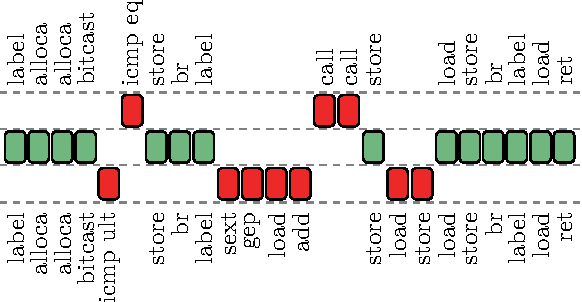
\includegraphics[width=0.75\linewidth]{src/background/figs/opcode-align.pdf}
  %\caption{An example of a sequence alignment between two real functions extracted from the \text{400.perlbench} benchmark.}
  \caption{The sequence alignment between two functions, identifying the equivalent segments of code (green in the center) and the non-equivalent ones (red at the sides).}
  \label{fig:opcode-align}
\end{figure}

Specifically for function-merging, we are concerned with the alphabet
consisting of all possible typed instructions and labels.
Every linearized function represents a sequence derived from this alphabet.
We explain the equivalence relation used for this alphabet in the next section.
Although we only consider pair-wise alignments, the technique would also work
for multi-sequences.

%We describe the equivalence relation between two predicated values in two
%separate cases, namely, the equivalence between instructions and the
%equivalence between labels.
%Labels are always considered equivalent.
%Two instructions are equivalent if their opcode are semantically equivalent,
%but not necessarily the same, and they both have types that can be bitcasted in
%a losslessly way from on to the other.
%This also includes making sure that there is no conflict regarding memory
%alignment when handling pointers.
%No additional restriction is imposed on the operands of the two instructions
%being compared for equivalence.
%Whenever two operands cannot be statically proved to represent the same value,
%a select instruction can be used to distinguish between the execution of two
%functions being merged.
%For function calls, the type equivalence requires that both instructions have
%identical function types, i.e., both called functions must have an identical
%return type and an identical list of parameter types.

%There is a vast literature on algorithms for performing sequence alignment,
%especially in the context of molecular biology.
%These algorithms range from optimal algorithms based on dynamic programming to
%probabilistic models that do not guarantee
%optimality~\cite{needleman70,smith81,carrillo88,hickey11}.
Our work uses the Needleman-Wunsch algorithm~\cite{needleman70} to perform sequence alignment.
This algorithm gives an alignment that is guaranteed to be optimal for a given scoring scheme~\cite{higgins89},
however, other algorithms could also be used with different performance and memory usage trade-offs~\cite{needleman70,smith81,carrillo88,hickey11}.
Different alignments would produce different but valid merged functions.

The Needleman-Wunsch algorithm~\cite{needleman70} is based on dynamic programming and consists of two main steps. First, it builds a \textit{similarity matrix}, based on a scoring scheme, which assigns weights
for matches, mismatches, and \textit{gaps} (blank characters). Afterwards, a backward traversal is performed on the similarity matrix, in
order to reconstruct the final alignment by maximizing the total score. We use a standard scoring scheme for the Needleman-Wunsch algorithm
that rewards matches and equally penalizes mismatches and gaps.
